\section{Algebraic engines, SAT, and linear algebra}\label{sec:solvers}

The solver programme is broader than a single F4 implementation. It
includes Boolean matrix F4, signature/F5 variants, inherited elimination
over assignment trees, geometry-assisted F6-IC, prime-field F4, tower
arithmetic, sparse and dense kernels, Four-Russians elimination, SAT/XOR
encodings, linear-row harvesting, GPU offload and destination matrix
solvers. These are reusable instruments, even where the current ECDLP
pipeline prefers an enumerative oracle.\src{GB}\src{CA-README}

\subsection{Inherited elimination and the accounting lesson}

Inherited F4 carries a parent's reduced information into a child partial
assignment rather than constructing a fresh Macaulay matrix at every
node. On the identical-tree K13 and random-13 panels, the record reports
matrix-work reductions of 198.6 and 222.1 relative to matrix F4. F5's
word-XOR ratios against F4 are about 0.6465 and 0.6414. These are
specific stage counters on particular systems, not a claim that every
F4 task is hundreds of times faster.\src{GB}\src{PRIOR}

F6-IC adds factor-base domain pruning and meet-in-the-middle leaves.
Its word-XOR count is lower than inherited F4, and its relation stage can
be faster. Once the leaf geometry and batched additions are charged,
however, the older complete-cost study reports F6-IC costs 64.6--68.8
times inherited F4 at degree 13 and 1,303--1,353 times at degree 19.
The saved algebraic counter moved work into another phase. That is an
accounting loss on those workloads, not a reason to delete the stage
measurement or to assume every future geometry-assisted engine must
lose.

The engine audit also found a prime-field soundness bug, contract
defects and latent holes. Its regression and brute-force comparisons are
part of the progress: a fast engine that can discard a real root is not
an acceptable oracle. Correctness must cover both positive witnesses and
negative decisions, not just the final answer on favourable targets.

\subsection{What the external comparisons establish}

The prime-field F4 work reports 29.8--54.1 improvements over its
predecessor on square generic systems, with msolve/ours ratios
0.96--1.22 in the recorded single-thread comparison. Reduced bases are
checked against external tools. This is a useful example of making the
external baseline explicit. It is not a comprehensive fastest-solver
claim over other degrees, fields, orderings, thread counts or hardware.
\src{FP-F4}

Task identity is equally important. Deciding whether a Boolean system
has an admissible root, extracting a few linear consequences, and
computing a complete reduced basis are different jobs. The fact that a
specialised oracle decides a target in milliseconds while a general CAS
spends seconds producing a full basis does not by itself establish a
corresponding engine speedup on equal outputs. The portfolio's newer
external-comparison rule requires the same inputs, outputs and host,
and names missing external tools rather than selecting a convenient
slower reference.\src{C-RULES}\src{PRIOR}

\subsection{GPU results: real acceleration and a negative deployment result}

The RTX 5090 experiment is particularly informative because it records
both. A degree-six Macaulay task with 168,363 rows and 188,203 columns
takes 425.8 seconds for host build plus elimination and 5.70 seconds for
device build plus elimination, a recorded factor of 74.7 on that pod.
Another degree-six matrix improves 25.5 times. Ranks, refutations and
pinned variables agree. The device column includes first-use CUDA/NVRTC
cost in the first elimination; separate upload and kernel times are also
reported.\src{F4-GPU}

Yet the small per-node device decider does not beat the production
inherited host engine. On its fixed 1,024-target oracle panel, the GPU
path takes 5.57 seconds while the default inherited host path takes
1.25 seconds. The GPU is useful on the large matrices; the better host
algorithm wins on the small repeated systems. A proposed deployment
should use this result to decide where to offload, rather than project
the large-matrix factor onto the whole IC pipeline.

The H100 follow-up records a kept tiled update, 1.11--1.49 times faster
on the measured matrices, and a reverted merged-basis panel that is
1.5--5.3 times slower. Upload costs remain. This is a concrete record of
an optimisation search with a retained unsuccessful arm.\src{F4-PANEL}

\begin{figure}[htbp]
\centering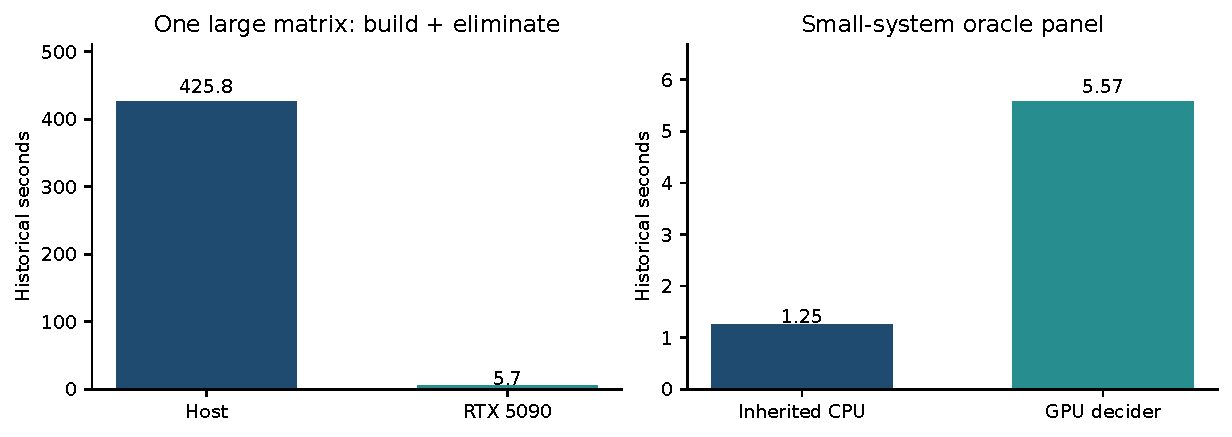
\includegraphics[width=\linewidth]{figures/gpu-stages.pdf}
\caption{Two different boundaries in the RTX 5090 study. Left: one large
degree-six matrix, host and device build plus elimination. Right: the
small-system oracle panel, where the inherited CPU engine is faster than
the GPU decider. Historical wall observations, not a new measurement or
an end-to-end ECDLP speedup. Source: \src{F4-GPU}.}
\end{figure}

The root-finding CUDA kernel is a separate case: the cited implementation
is host-emulated, with no GPU measurement in that study. Its validation
cannot inherit the F4 kernel's hardware evidence merely because both use
CUDA.\src{RF-GPU}

\subsection{Factor-base geometry and empirical solver selection}

The cryptanalysis product-profile study measures 656 factor bases from
seven families over nine fields. For two-summand systems it fits the
empirical rule
\[
 e=n-\dim V-\dim V^{(2)},\qquad
 D=2+[e<-3.5]+[e<-8.5],
\]
with mean absolute error 0.06 degrees, or 0.08 when leaving out each
field size. This is a fitted rule on that dataset, not a proved
degree law for growing parameters. In selected cells, geometric
progression bases reduce query cost 15--40 times relative to random
bases while leaving yield similar.\src{HEUR}

The three-summand comparison shows why formulation is another research
lever. Direct coordinates and symmetric variables live in different
product spaces. Minimising the dimensions of $V^{(k)}$ can reduce the
number of symmetric unknowns even at the same solving degree. The
report explicitly labels these rows PDP-stage profiles and keeps their
candidate identity unset until a calibrated complete pipeline exists.

It also identifies a practical stopping condition: a relation collector
can wait forever for full rank when the attainable matrix rank is one
less than the number of columns. Solving modulo the known kernel and
verifying the target is different from assuming that another dependent
row will repair it. This is a concrete lesson about implementations, not
only asymptotic analysis.

\subsection{Linear algebra and harvested information}

Linear algebra is the phase most likely to invalidate a relation-only
crossover. The residual-walk record documents a claimed relation-phase
crossing that disappears after matrix cost is included. Sparse filtering,
structured Gaussian elimination, Lanczos, Wiedemann and block Wiedemann
are therefore method components, not cleanup after the interesting part.
\src{RESIDUAL}

The later genus-three experiments compare complete solvers after changing
large-prime handling and matrix strategy. One structured-elimination and
Wiedemann route has recorded complete candidate/incumbent ratio 0.653
[0.647,0.660] at $q=2^{20}$, with 474 verified logs in its panel.
Its linear-algebra constant improves while the fitted exponent of that
phase rises. A subsequent block-Wiedemann change gives about 0.945 at
$2^{21}$; a combined schedule and solver reaches 0.605 of the earlier
round-one baseline. These factors belong to their named comparison
chains and are not multiplied into an invented cumulative factor on the
prime-field ECDLP.\src{ROUND2}

Linear-row harvesting is another modest, testable gain. The recorded
root-set panel has zero failures on 96 comparisons; selected oracle
cells improve about 1.07--1.17 times. The report also states where the
bench gain fails to carry into production because the production solve
stops at its first accepted root. The exact stopping policy is part of
the workload definition.
